\addcontentsline{toc}{section}{Appendices}
\section*{Appendices}

% Define custom colors using hex codes
\definecolor{YOLOv5Color}{HTML}{4F97BA} % gray
\definecolor{YOLOv6Color}{HTML}{37718e} % blue
\definecolor{YOLOXColor}{HTML}{254e70} % green
\definecolor{GYoloColor}{HTML}{c33c54} % red

\subsection*{A}

% Latency Graph
\begin{figure}[htbp]
    \centering
    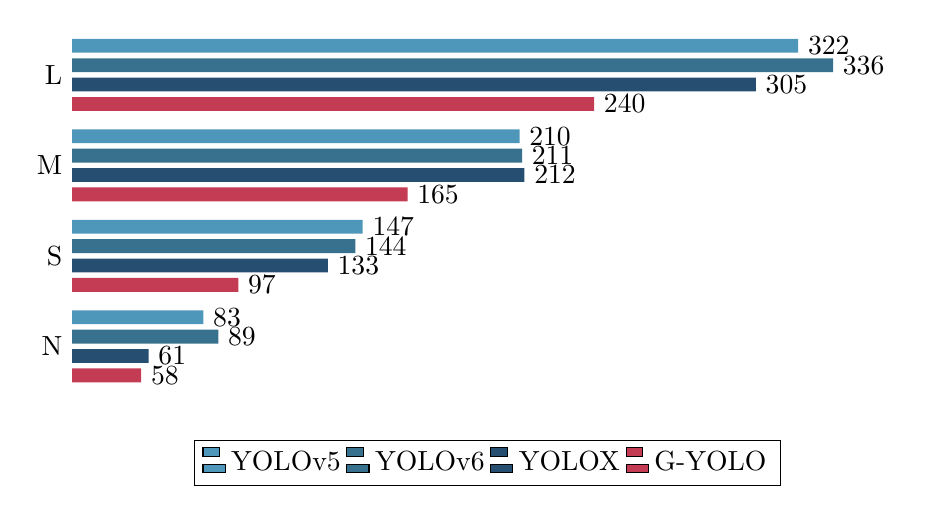
\begin{tikzpicture}
        \begin{axis}[
            xbar,
            y axis line style = { opacity = 0 },
            axis x line       = none,
            tickwidth         = 0pt,
            enlarge y limits  = 0.15,
            symbolic y coords={N, S, M, L},
            ytick=data,
            nodes near coords,
            xlabel={Latency (ms)},
            width=\textwidth,
            height=0.5\textwidth,
            bar width=5pt,
            legend style={at={(0.5,-0.15)},
                anchor=north,legend columns=-1},
            reverse legend,
        ]
        % Define custom colors
        \addplot [draw=none, fill=GYoloColor] coordinates {(58,N) (97,S) (165,M) (240,L)}; % G-YOLO
        \addplot [draw=none, fill=YOLOXColor] coordinates {(61,N) (133,S) (212,M) (305,L)}; % YOLOX
        \addplot [draw=none, fill=YOLOv6Color] coordinates {(89,N) (144,S) (211,M) (336,L)}; % YOLOv6
        \addplot [draw=none, fill=YOLOv5Color] coordinates {(83,N) (147,S) (210,M) (322,L)}; % YOLOv5
        \legend{G-YOLO, YOLOX, YOLOv6, YOLOv5}
        \end{axis}
    \end{tikzpicture}
    \caption{Latency comparison between various YOLO and G-YOLO models on VOC dataset.}
    \label{fig:latency_comparison_voc}
\end{figure}

% mAP Graph
\begin{figure}[htbp]
    \centering
    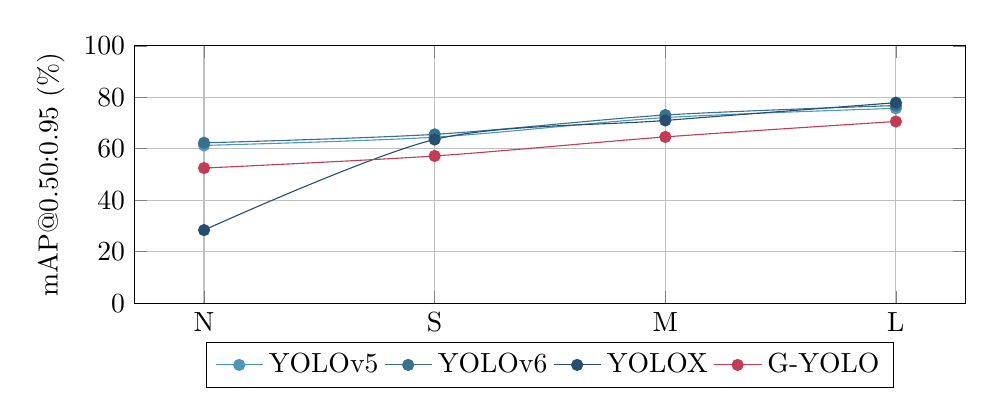
\begin{tikzpicture}
        \begin{axis}[
            xlabel={Model Variant},
            ylabel={mAP@0.50:0.95 (\%)},
            xtick={1, 2, 3, 4},
            xticklabels={N, S, M, L},
            width=\textwidth,
            height=0.4\textwidth,
            legend style={at={(0.5,-0.15)},
                anchor=north,legend columns=-1},
            ymin=0, ymax=100,
            grid=major,
            smooth
        ]

        \addplot[color=YOLOv5Color, mark=*] coordinates {
            (1, 61.3)
            (2, 64.5)
            (3, 72.1)
            (4, 75.7)
        };
        \addplot[color=YOLOv6Color, mark=*] coordinates {
            (1, 62.3)
            (2, 65.6)
            (3, 73.1)
            (4, 76.8)
        };
        \addplot[color=YOLOXColor, mark=*] coordinates {
            (1, 28.4)
            (2, 63.6)
            (3, 71.0)
            (4, 77.9)
        };
        \addplot[color=GYoloColor, mark=*] coordinates {
            (1, 52.5)
            (2, 57.2)
            (3, 64.6)
            (4, 70.6)
        };

        \legend{YOLOv5, YOLOv6, YOLOX, G-YOLO}
        \end{axis}
    \end{tikzpicture}
    \caption{mAP comparison between various YOLO and G-YOLO models on VOC dataset.}
    \label{fig:map_comparison_voc}
\end{figure}

% Latency Graph for RoadSec
\begin{figure}[htbp]
    \centering
    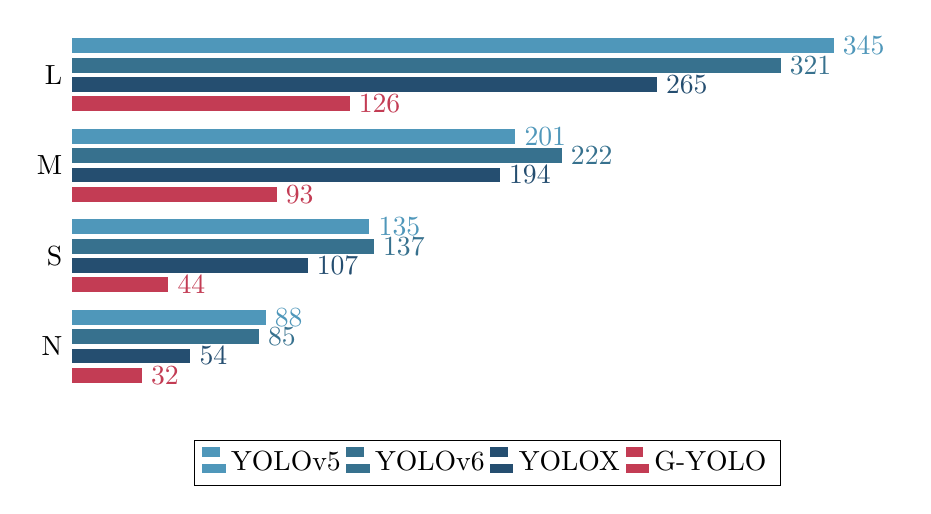
\begin{tikzpicture}
        \begin{axis}[
            xbar,
            y axis line style = { opacity = 0 },
            axis x line       = none,
            tickwidth         = 0pt,
            enlarge y limits  = 0.15,
            symbolic y coords={N, S, M, L},
            ytick=data,
            nodes near coords,
            xlabel={Latency (ms)},
            width=\textwidth,
            height=0.5\textwidth,
            bar width=5pt,
            legend style={at={(0.5,-0.15)},
                anchor=north,legend columns=-1},
            reverse legend,
            xticklabel style={/pgf/number format/1000 sep=\,},
        ]
        \addplot[color=GYoloColor, fill=GYoloColor] coordinates {(32,N) (44,S) (93,M) (126,L)};
        \addplot[color=YOLOXColor, fill=YOLOXColor] coordinates {(54,N) (107,S) (194,M) (265,L)};
        \addplot[color=YOLOv6Color, fill=YOLOv6Color] coordinates {(85,N) (137,S) (222,M) (321,L)};
        \addplot[color=YOLOv5Color, fill=YOLOv5Color] coordinates {(88,N) (135,S) (201,M) (345,L)};
        \legend{G-YOLO, YOLOX, YOLOv6, YOLOv5}
        \end{axis}
    \end{tikzpicture}
    \caption{Latency comparison between various YOLO and G-YOLO models on RoadSec dataset.}
    \label{fig:latency_comparison_roadsec}
\end{figure}

% mAP Graph for RoadSec
\begin{figure}[htbp]
    \centering
    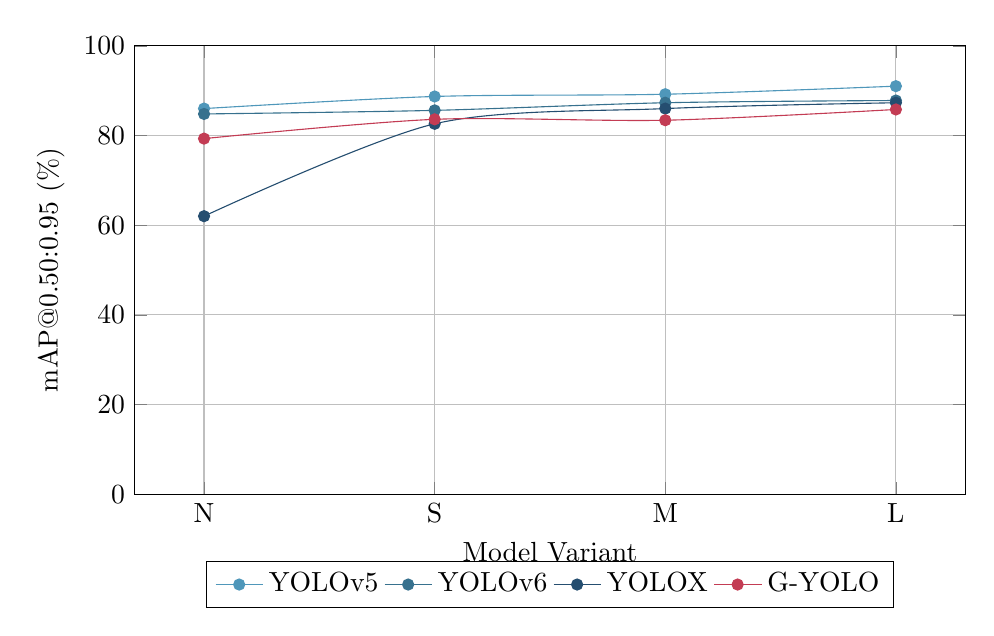
\begin{tikzpicture}
        \begin{axis}[
            xlabel={Model Variant},
            ylabel={mAP@0.50:0.95 (\%)},
            xtick={1, 2, 3, 4},
            xticklabels={N, S, M, L},
            width=\textwidth,
            height=0.6\textwidth,
            legend style={at={(0.5,-0.15)},
                anchor=north,legend columns=-1},
            ymin=0, ymax=100,
            grid=major,
            smooth
        ]

        \addplot[color=YOLOv5Color, mark=*] coordinates {
            (1, 86.0)
            (2, 88.7)
            (3, 89.2)
            (4, 91.0)
        };
        \addplot[color=YOLOv6Color, mark=*] coordinates {
            (1, 84.8)
            (2, 85.6)
            (3, 87.3)
            (4, 87.8)
        };
        \addplot[color=YOLOXColor, mark=*] coordinates {
            (1, 62.0)
            (2, 82.6)
            (3, 86.0)
            (4, 87.3)
        };
        \addplot[color=GYoloColor, mark=*] coordinates {
            (1, 79.3)
            (2, 83.6)
            (3, 83.4)
            (4, 85.8)
        };

        \legend{YOLOv5, YOLOv6, YOLOX, G-YOLO}
        \end{axis}
    \end{tikzpicture}
    \caption{mAP comparison between various YOLO and G-YOLO models on RoadSec dataset.}
    \label{fig:map_comparison_roadsec}
\end{figure}


\begin{figure}[htbp]
    \centering
    \begin{minipage}[b]{0.45\textwidth}
        \centering
        \includegraphics[width=\textwidth]{figures/Picture1.png}
        \caption{Output of G-YOLOv6}
        \label{fig:our_method}
    \end{minipage}
    \hfill
    \begin{minipage}[b]{0.45\textwidth}
        \centering
        \includegraphics[width=\textwidth]{figures/Picture2.png}
        \caption{Output of YOLOv6 N}
        \label{fig:yolov6}
    \end{minipage}
    \caption{Comparison of Object Detection Outputs. The image on the left shows the result of our method, achieving over 30 FPS consistently on the Jetson TX2. The image on the right shows the result of the YOLOv6 N model, achieving an average of 11 FPS. Both models provide very similar results in terms of detection accuracy.}
    \label{fig:comparison}
\end{figure}

\clearpage

\subsection*{B}

\clearpage
